\documentclass{article}
\usepackage[utf8]{inputenc}
\usepackage{graphicx}
\usepackage{amsmath}
\usepackage{indentfirst}
\usepackage[a4paper, total={7in, 10in}]{geometry}
\graphicspath{ {./../res/} }

\title{Nanoparticles size estimation throught Mie resonances}
\author{Neven Gentil}
\date{April 2022}

\begin{document}

\maketitle

\twocolumn

\section{Introduction}

Hello LaTeX World!

Hello, here is some text without a meaning. This text should show what a printed text will look like at this place.
If you read this text, you will get no information. Really? Is there no information? Is there.Hello LaTeX World!
Hello, here is some text without a meaning. This text should show what a printed text will look like at this place.
If you read this text, you will get no information. Really? Is there no information? Is there.
\begin{figure}[h]
    \centering
    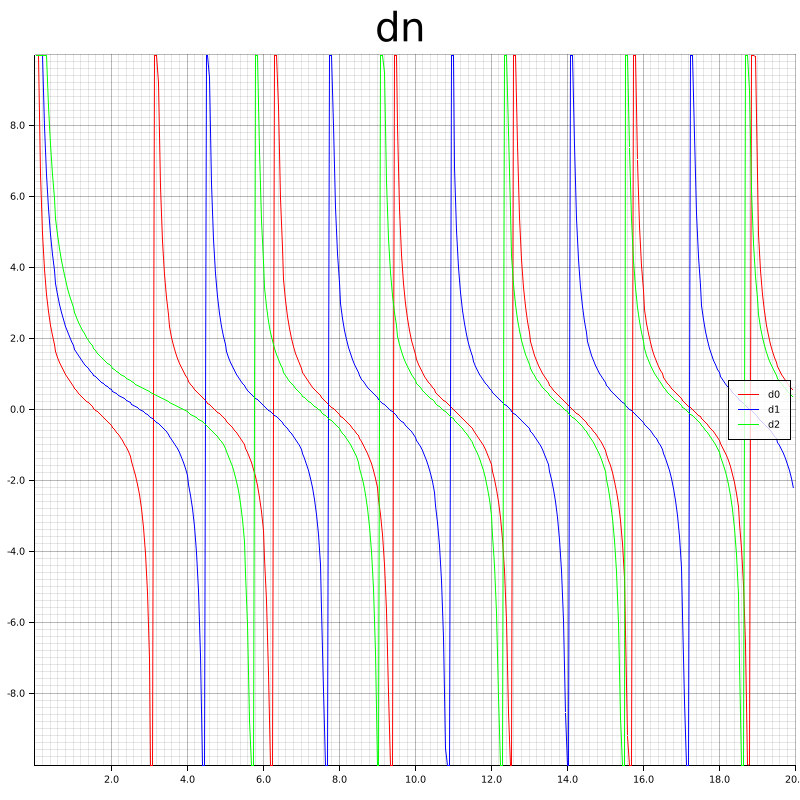
\includegraphics[width=0.5\textwidth, height=0.25\textheight]{dn.png}
    \caption{a nice plot}
    \label{fig:dn_plot}
\end{figure}
Hello LaTeX World!
Hello, here is some text without a meaning. This text should show what a printed text will look like at this place.
If you read this text, you will get no information. Really? Is there no information? Is there.Hello LaTeX World!
Hello, here is some text without a meaning. This text should show what a printed text will look like at this place.
If you read this text, you will get no information. Really? Is there no information? Is there.
\section{EXP}
\begin{figure}[h]
    \centering
    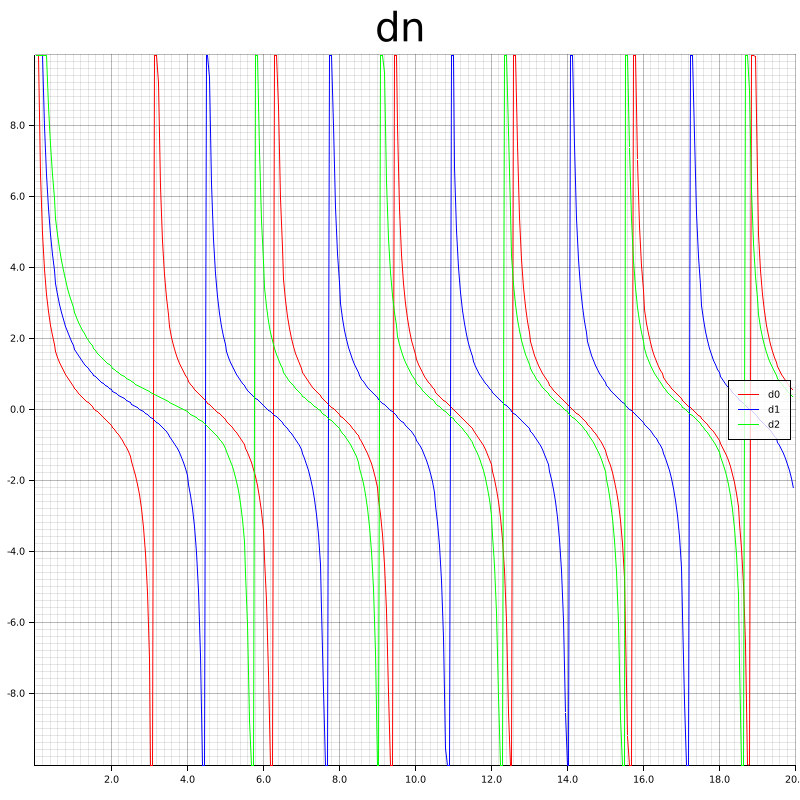
\includegraphics[width=0.5\textwidth, height=0.25\textheight]{dn.png}
    \caption{a nice plot}
    \label{fig:dn_plot}
\end{figure}
\begin{equation} \label{eq:haha}
\begin{aligned}
    E = m*2+4*x-4 / 5000.0 + 4000000 \\
    - 7777777 - 5 + 7777 + 4000000= 80a
\end{aligned}
\end{equation}
Hello LaTeX World! Eq \ref{eq:haha} is...
Hello, here is some text without a meaning. This text should show what a printed text will look like at this place.
If you read this text, you will get no information. Really? Is there no information? Is there.Hello LaTeX World!
Hello, here is some text without a meaning. This text should show what a printed text will look like at this place.
If you read this text, you will get no information. Really? Is there no information? Is there.
Hello LaTeX World!
Hello, here is some text without a meaning. This text should show what a printed text will look like at this place.
If you read this text, you will get no information. Really? Is there no information? Is there.Hello LaTeX World!
Hello, here is some text without a meaning. This text should show what a printed text will look like at this place.
If you read this text, you will get no information. Really? Is there no information? Is there.
Hello LaTeX World!
Hello, here is some text without a meaning. This text should show what a printed text will look like at this place.
If you read this text, you will get no information. Really? Is there no information? Is there.Hello LaTeX World!
Hello, here is some text without a meaning. This text should show what a printed text will look like at this place.
If you read this text, you will get no information. Really? Is there no information? Is there.
Hello LaTeX World!
Hello, here is some text without a meaning. This text should show what a printed text will look like at this place.
If you read this text, you will get no information. Really? Is there no information? Is there.Hello LaTeX World!
Hello, here is some text without a meaning. This text should show what a printed text will look like at this place.
If you read this text, you will get no information. Really? Is there no information? Is there.

\newpage

\section{Theorie}

First of all, let's describe the general composition of our problem: given an arbitrary particle droped in a certain medium, we hit it with a monochromatic light. With a fixed size and other specifics parameters for electromagnetic materials like the permeability $\mu$ or the complex refractive index $N$, our objective is to theoretically compute the electromagntic field for the medium surrounding the particle and inside this particle itself.

Let's start with an arbitrary electromagntic field represented by the couple of \textit{monochromatic} vector field $(\textbf{E}, \textbf{H})$ which satisfies the Maxwell equations:
\begin{align}
\nabla \cdot \textbf{E} &= 0\\
\nabla \cdot \textbf{H} &= 0\\
\nabla \times \textbf{E} &= i\omega \mu \textbf{H} \label{eq:rot_e} \\
\nabla \times \textbf{H} &= -i\omega \epsilon \textbf{E} \label{eq:rot_h}
\end{align}
Given the relation $k^{2} = \omega ^{2}\epsilon \mu$ and the following formula:
\begin{align}\label{eq:rot_rot_a}
\nabla \times (\nabla \times \textbf{A}) = \nabla (\nabla \cdot \textbf{A}) - \nabla \cdot (\nabla \textbf{A})
\end{align}
we obtain a couple of \textit{vector wave equation}:
\begin{align}
\nabla ^{2} \textbf{E} + k^{2}\textbf{E}&=0\\
\nabla ^{2} \textbf{H} + k^{2}\textbf{H}&=0
\end{align}
where $\nabla ^{2}$ is the vector Laplace operator, that is to say, we explicitly have $\Delta \textbf{A} = \nabla ^{2} \textbf{A} = (\nabla \cdot \nabla) \textbf{A}$.

An important thing to notice is that any vector field with zero divergence and satisfying the vector wave equation is a valid electric/magnetic field where we can obtain the corresponding magnetic/electric field by the curl (\ref{eq:rot_e})/(\ref{eq:rot_h}).

In this way, it is possible to create a vector function $\textbf{M}$ depending on a scalar function $\psi$ and an arbitrary constant vector $\textbf{c}$:
\begin{align}
\textbf{M} = \nabla \times (\textbf{c}\psi)
\end{align}
where \textbf{M} directly satisfies the condition $\nabla \cdot \textbf{M} = 0$. If we replace the expression of \textbf{M} in the vector wave equation, and thanks to (\ref{eq:rot_rot_a}), we easily obtain:
\begin{align}
\nabla ^{2} \textbf{M} + k^{2}\textbf{M} = \nabla \times [\textbf{c}(\nabla ^{2} \psi + k^{2}\psi)]
\end{align}
To satisfy the vector wave equation, $\psi$ should also satisfy the equivalent scalar wave equation:
\begin{align}\label{eq:psi_wave_eq}
\nabla ^{2} \psi + k^{2}\psi = 0
\end{align}
where, this time, $\nabla ^{2}$ is the scalar Laplace operator. By the way, as described above, if we denote $\nabla \times \textbf{N} = k \textbf{M}$, we have the perpendicular vector field of the associated artificial one, also satisfying the vector wave equation. Finally, we created the vector harmonics $\textbf{M}$ and $\textbf{N}$ with the scalar generating function $\psi$ associated to our initial electromagntic field.

The main idea to compute all solutions required is the following: given an incident electromagntic field, we use the boundary conditions on the surface of our particle to get all fields resulting from interaction. Thereby, it could be interesting to use the spherical polar coordinates during the calculation and particularly to express the boundary conditions. That is why we have constructed the vector harmonics above. Indeed, if we replace the constant vector $\textbf{c}$ by the radial coordinate $\textbf{r}$, $\textbf{M}$ is always a solution of the vector wave equation but, this time, for the spherical polar coordinates linked to the particle. In this way, from (\ref{eq:psi_wave_eq}), we obtain:
\begin{equation}\label{eq:wave_sph}
\begin{aligned}
\frac{1}{r^{2}}\frac{\partial }{\partial r}(r^{2}\frac{\partial \psi}{\partial r}) + \\ 
\frac{1}{r^{2}sin(\theta)}\frac{\partial }{\partial \theta}(sin(\theta)\frac{\partial \psi}{\partial \theta}) + \\
\frac{1}{r^{2}sin(\theta)}\frac{\partial^{2} \psi}{\partial^{2} \phi} + \\
k^{2}\psi = 0
\end{aligned}
\end{equation}
Obviously, from the previous formula, we can separate each variable to create $\psi$:
\begin{align}\label{eq:psi_r_t_p}
\psi(r, \theta, \phi) = R(r)\Theta(\theta)\Phi(\phi)
\end{align}
Thereby, when substitued (\ref{eq:psi_r_t_p}) into (\ref{eq:wave_sph}), we obtain three different equations, depending respectively on $r$, $\theta$ and $\phi$ which might be solved separately.

Finally, this kind of generating function $\psi$ satisfying the scalar wave equation (\ref{eq:psi_wave_eq}) is expressed in two \textit{even} ($\psi_{e}$) and \textit{odd} ($\psi_{o}$) functions as follow:
\begin{align}
\psi_{emn}&=cos(m\phi)P_{n}^{m}(cos\theta)z_{n}(kr)\\
\psi_{omn}&=sin(m\phi)P_{n}^{m}(cos\theta)z_{n}(kr)
\end{align}
where the parity of our original function is led by the $cosinus$ and $sinus$ attached with the $\phi$ variable and the \textit{angle-dependant} $m$ variable. 

The other angular part described by $\theta$ , as a \textit{Legendre's differential equation}, is solved by the \textit{associated Legendre functions} of the first kind $P_{n}^{m}(cos\theta)$ orthogonally defined on the $n$ variable. 

Moreover, the radial part, described by $r$, might be reintroduced as follow:
\begin{align}
\rho\frac{d }{d\rho}(\rho\frac{d Z}{d\rho})+[\rho^{2}-(n+\frac{1}{2})^{2}]Z=0
\end{align}
where we assume that $\rho=kr$ and $Z=R\sqrt{\rho}$. Thereby, to solve the previous equation, we can use any linear combination of the spherical Bessel functions $j_{n}$, $y_{n}$, $h^{(1)}_{n}=j_{n}+iy_{n}$ or $h^{(2)}_{n}=j_{n}-iy_{n}$: we named this kind of combination $z_{n}$.

Note that $m$ and $n$ are produced by subsidiary conditions when obtaining these three equations by rewriting (\ref{eq:wave_sph}) with separate variables: it is inherent to our physical assumptions.

In the end, we can retrieve our initial vector spherical harmonics generated by $\psi_{emn}$ or $\psi_{omn}$:
\begin{align}
\textbf{M}_{emn}=\nabla \times (\textbf{r}\psi_{emn})\\
\textbf{M}_{omn}=\nabla \times (\textbf{r}\psi_{omn})\\
\textbf{N}_{emn}=\frac{\nabla \times \textbf{M}_{emn}}{k}\\
\textbf{N}_{omn}=\frac{\nabla \times \textbf{M}_{omn}}{k}
\end{align}

At this point of the theorie, it is still possible to restrain our hypothesis and more precisely the shape of the incident light. Let's consider a planar incident electromagnetic wave $E_{i}$. Now, we can easily describe this wave in terms of vector spherical harmonics:
\begin{equation}\label{eq:ei_harmo}
\begin{aligned}
    \textbf{E}_{i}=\sum_{m=0}^{\infty }\sum_{n=m}^{\infty }B_{emn}\textbf{M}_{emn}+B_{omn}\textbf{M}_{omn}\\
+A_{emn}\textbf{N}_{emn}+A_{omn}\textbf{N}_{omn}
\end{aligned}
\end{equation}
Thanks to the orthogonality of all the vector spherical harmonics which could be demonstrated throught properties from $cos(m\phi)$, $sin(m\phi)$ and $P_{n}^{m}(cos\theta)$, we easily exctract each factor of this linear summation (\ref{eq:ei_harmo}):
\begin{align}\label{eq:bemn}
\textbf{B}_{emn}=\frac{\int_{0}^{2\pi}\int_{0}^{\pi}\textbf{E}_{i}\cdot \textbf{M}_{emn}sin\theta d\theta d\phi}{\int_{0}^{2\pi}\int_{0}^{\pi}|\textbf{M}_{emn}|^{2}sin\theta d\theta d\phi}
\end{align}
with here, for instance, the first coefficient. With the orthogonality and \ref{eq:bemn} of the sine and cosine, we can also demonstrate that $B_{emn}$ and $A_{omn}$ vanishe for all $m$ and $n$. Then, for the same reason, $B_{omn}$ and $A_{emn}$ are nonzero only for $m=1$. Moreover, regarding their behavior and our physical assumptions, we can select the spherical Bessel function replacing $z_{n}$: we choose $j_{n}$ for its finite values close to $r=0$ and denote it as $^{(1)}$ for the associated vector spherical harmonics. Finally, we obtain:
\begin{align}
\textbf{E}_{i}=\sum_{n=1}^{\infty }B_{o1n}\textbf{M}^{(1)}_{o1n} + A_{e1n}\textbf{N}^{(1)}_{e1n}
\end{align}
Afterward, thanks to a bunch of properties from the associated Legendre functions, we deduce explicitly these two remaining factors $B_{o1n}$ and $A_{e1n}$:
\begin{align}
\textbf{E}_{i}=E_{0}\sum_{n=1}^{\infty }i^{n}\frac{2n+1}{n(n+1)}(\textbf{M}^{(1)}_{o1n} - i\textbf{N}^{(1)}_{e1n})
\end{align}
Obviously, it is possible to calculate the perpendicular magnetic field $H_{i}$ with the curl (\ref{eq:rot_e}).

At this point, we have enough equation relative to the incident plane wave to apply the following boundary conditions:
\begin{align}
(\textbf{E}_{i} + \textbf{E}_{s} - \textbf{E}_{I}) \times \overrightarrow{e_{r}} &= 0\\
(\textbf{H}_{i} + \textbf{H}_{s} - \textbf{H}_{I}) \times \overrightarrow{e_{r}} &= 0
\end{align}
where $(\textbf{E}_{s}, \textbf{H}_{s})$ and $(\textbf{E}_{I}, \textbf{H}_{I})$ are respectively the scattering and internal electromagnetic field resulting from the interaction between the incident field and our particle. Then, we assume that these last fields have the same mathematical shape, when developped in vector spherical harmonics, than $(\textbf{E}_{i}, \textbf{H}_{i})$; that is to say, the scattering and internal field are linearly dependant from the incident field up to some factors taking into account the behavior of $j_{n}$ at the boundary of our particle:
\begin{align}
\textbf{E}_{I}&=\sum_{n=1}^{\infty }E_{n}(c_{n}\textbf{M}^{(1)}_{o1n} - id_{n}\textbf{N}^{(1)}_{e1n})\\
\textbf{H}_{I}&=\frac{-k_{I}}{\omega\mu_{I}}\sum_{n=1}^{\infty }E_{n}(d_{n}\textbf{M}^{(1)}_{e1n} + ic_{n}\textbf{N}^{(1)}_{o1n})\\
\textbf{E}_{s}&=\sum_{n=1}^{\infty }E_{n}(ia_{n}\textbf{N}^{(3)}_{e1n} - b_{n}\textbf{M}^{(3)}_{o1n})\\
\textbf{H}_{s}&=\frac{k}{\omega\mu}\sum_{n=1}^{\infty }E_{n}(ib_{n}\textbf{N}^{(3)}_{o1n} + a_{n}\textbf{M}^{(3)}_{e1n})
\end{align}
Note that $^{(3)}$ means we use the spherical Bessel function of the third kind $h^{(1)}_{n}$ and $\textbf{H}_{X}$ as the factors than $\textbf{E}_{X}$ due to the curl (\ref{eq:rot_e}).

\section{Simulations}

\section{Experiments}

\section{Conclusion}

\end{document}